\graphicspath{{pict/}}
\DeclareGraphicsExtensions{.pdf,.png,.jpg}

\chapter{Конструкторский раздел}
\label{cha:design}

В данном разделе будет произведена конкретизация задач и проанализированы алгоритмы.

\section{IDEF0 Модель}

На рисунке 2.1 приведена IDEF0 функциональная модель вычисления редакционного расстояния.
\begin{figure}[H]
\centering
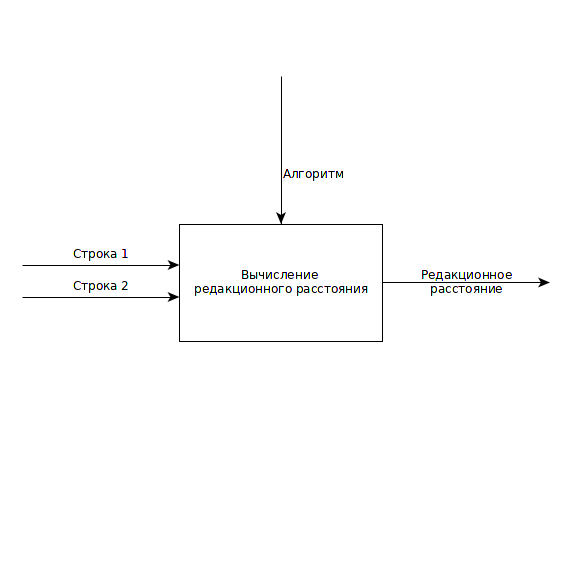
\includegraphics[scale=0.75]{1}
\caption{IDEF0 функциональная модель}
\end{figure}
\newpage

\section{Разработка алгоритмов}

\subsection{Алгоритм Вагнера-Фишера}
Алгоритм нахождения расстояния Вагнера-Фишера - это матричная реализация поиска расстояния Левенштейна, схема данного алгоритма приведена на рисунке 2.2.
\begin{figure}[H]
\centering
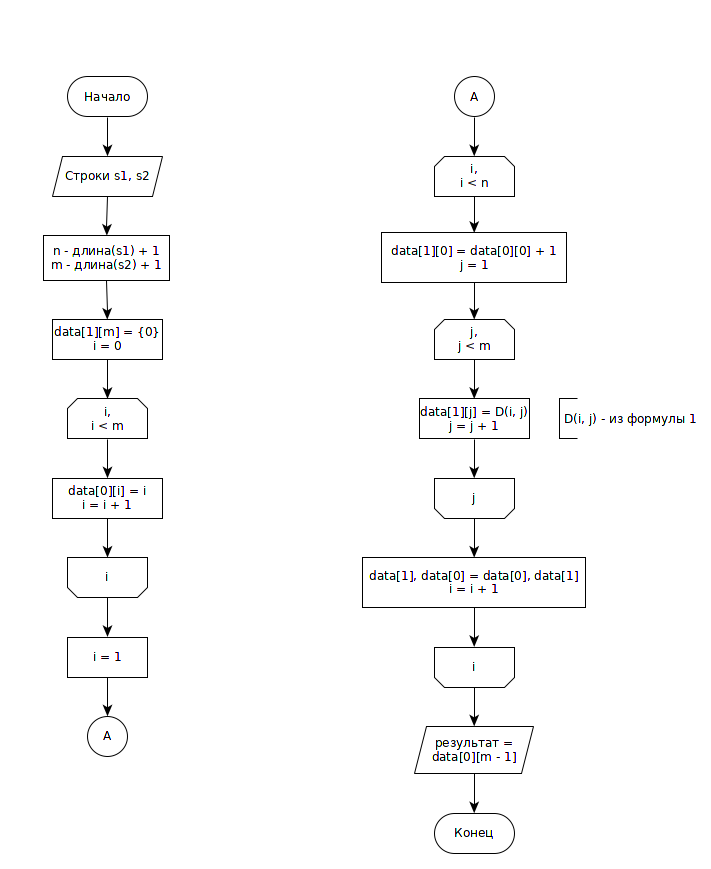
\includegraphics[scale=0.5]{3r}
\caption{Алгоритм Вагнера-Фишера}
\end{figure}

\subsection{Матричный алгоритм Дамерау-Левенштайна}
Матричный алгоритм нахождения расстояния Дамерау-Левенштайна - это модификация алгоритма Вагнера-Фишера, в котором добавлена операция транспозиции, схема данного алгоритма приведена на рисунке 2.3.

\begin{figure}[H]
\centering
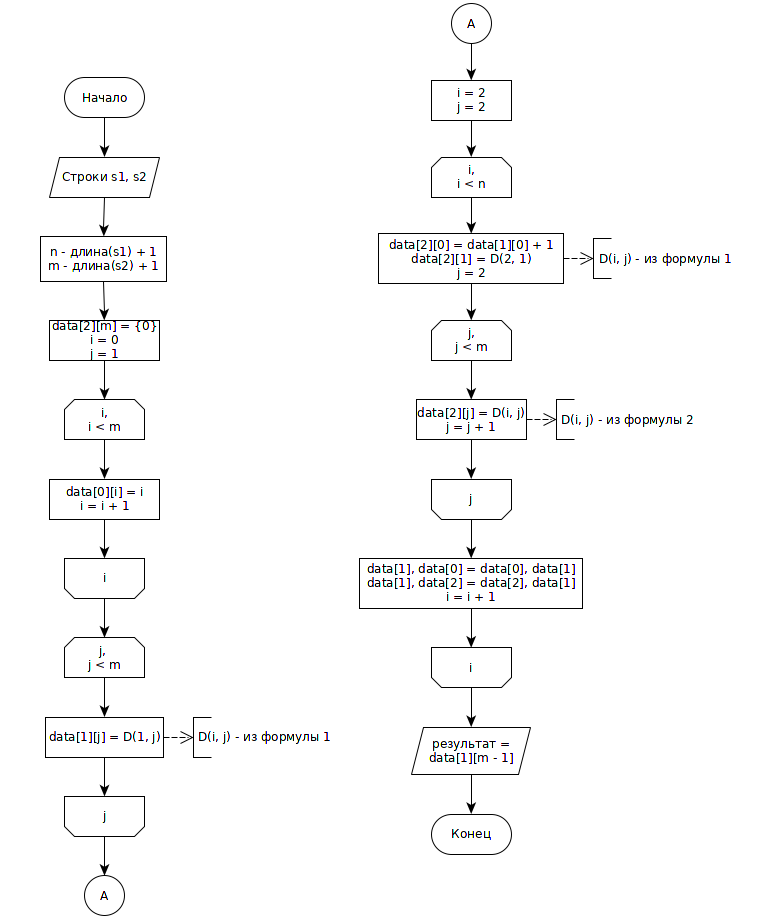
\includegraphics[scale=0.5]{trans}
\caption{Матричный алгоритм Дамерау-Левенштайна}
\end{figure}

\subsection{Рекурсивный алгоритм Дамерау-Левенштайна}
В рекурсивном алгоритме нахождения расстояния Дамерау-Левенштайна происходит поиск редакционного расстояния до тех пор, пока длина хотя бы одного из слов не равна 0, схема данного алгоритма приведена на рисунке 2.4
\begin{figure}[H]
\centering
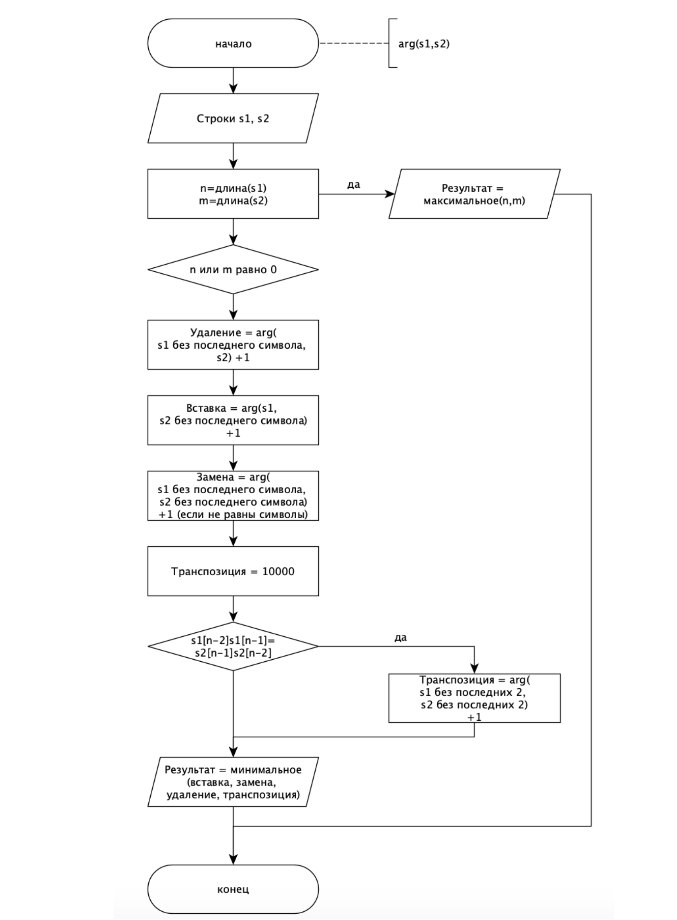
\includegraphics[scale=0.5]{rec}
\caption{Рекурсивный алгоритм Дамерау-Левенштайна}
\end{figure}

\section{Сравнительный анализ алгоритмов}

\subsection{Сравнение}

%Во время работы матричной реализации происходит обход матрицы размера \((S_1+1)\cdot(S_2+1)\), где \(S_1\) и \(S_2\) - длины обрабатываемых строк. Следовательно, данный алгоритм имеет сложность \(O(S_1\cdot{}S_2)\).
Матричная реализация имеет сложность $\Omega(mn)$, где m и n - это длины строк.
В самом коротком пути рекурсивный алгоритм нахождения расстояния Дамерау-Левенштейна имеет сложность $\Omega(4^{min(m,n)})$, а максимальная сложность $\Omega(4^{m + n + 1})$, где m и n - длины строк$.
%В реализации рекурсивного алгоритма присутствуют три точки входа в рекурсию. Это означает, что в худшем случае рекурсивный алгоритм Левенштейна будет иметь сложность  \(O(4^())\), где \(S\) - максимальная длина обрабатываемых слов.
\subsection{Вывод}

На основе вышеприведенного анализа можно сделать вывод о том, что матричная реализация быстрее рекурсивной при больших значениях длин строк.
